\section{Studying piecewise certificates on concrete one-dimensional examples}

Some useful examples to study are given in Tables~\ref{tab:kink-examples}
and~\ref{tab:curvature-examples}.

\begin{table}[t]
\centering
\caption{Piecewise linear certificates examples.}
\label{tab:kink-examples}
\begin{tabular}{lllll}
\hline
SDE & $V(x)$ & $D_t$ & $M_t$ & $K_t$ \\
\hline
$dX_t=dW_t$
&
$-|x|$
&
$0$
&
$\displaystyle \int_0^t -\operatorname{sgn}(X_s)\,dW_s$
&
$\displaystyle -L_t^0(X)$
\\[1.1em]

% $dX_t=dW_t$
% &
% $|x|$
% &
% $0$
% &
% $\displaystyle \int_0^t \operatorname{sgn}(X_s)\,dW_s$
% &
% $\displaystyle L_t^0(X)$
% \\[1.1em]

$dX_t=-X_t\,dt$
&
$|x|$
&
$\displaystyle -\int_0^t |X_s|\,ds$
&
$0$
&
$0$
\\
\hline
\end{tabular}
\end{table}

\begin{table}[t]
\centering
\caption{Piecewise $\mathcal{C}^2$ certificates examples.}
\label{tab:curvature-examples}
\resizebox{\textwidth}{!}{%
\begin{tabular}{llllll}
\hline
SDE & $V(x)$ & $D_t$ & $M_t$ & $C_t$ & $K_t$ \\
\hline
$dX_t=-\lambda X_t\,dt+\sigma\,dW_t$
&
$x^2$
&
$\displaystyle -2\lambda \int_0^t X_s^2\,ds$
&
$\displaystyle \int_0^t 2\sigma X_s\,dW_s$
&
$\displaystyle \sigma^2 t$
&
$0$
\\[1.1em]

$dX_t=dt+\sqrt{2}\,dW_t$
&
$\displaystyle x-\frac{x^2}{2}$
&
$\displaystyle \int_0^t (1-X_s)\,ds$
&
$\displaystyle \int_0^t (1-X_s)\sqrt{2}\,dW_s$
&
$\displaystyle -t$
&
$0$
\\[1.1em]

$dX_t=dW_t$
&
$\displaystyle
\begin{cases}
-\frac12 x^2, & x<0,\\
-x, & x\ge 0
\end{cases}$
&
$0$
&
$\displaystyle \int_0^t V'(X_s)\,dW_s$
&
$\displaystyle -\frac12\int_0^t \mathbf 1_{\{X_s<0\}}\,ds$
&
$\displaystyle -\frac12 L_t^0(X)$
\\
\hline
\end{tabular}%
}
\end{table}

\subsection{Ornstein--Uhlenbeck process in three parameter regimes}

Consider the Ornstein--Uhlenbeck process
\[
  dX_t=-\lambda X_t\,dt+\sigma\,dW_t
\]
with the quadratic certificate $V(x)=x^2$. Its generator is
\[
  \mathcal LV(x)=-2\lambda x^2+\sigma^2
  =-2\lambda\left(x^2-\frac{\sigma^2}{2\lambda}\right).
\]
Consequently, if
\[
  r=\frac{\sigma}{\sqrt{2\lambda}},
\]
then the generator is negative for $|x|>r$, zero for $|x|=r$, and positive
for $|x|<r$. The decomposition is
\[
  X_t^2-X_0^2
  =\underbrace{-2\lambda\int_0^t X_s^2\,ds}_{D_t}
  +\underbrace{2\sigma\int_0^t X_s\,dW_s}_{M_t}
  +\underbrace{\sigma^2t}_{C_t},
\]
with $K_t=0$.

Figure~\ref{fig:ou-terms} fixes $\lambda=1$ and $X_0=1$, and uses
$r=0.5$, $r=1$, and $r=1.5$. These choices make the initial generator
negative, zero, and positive, respectively. Moreover,
\[
  \mathbb E[X_t^2]
  =r^2+(X_0^2-r^2)e^{-2\lambda t},
\]
so the expected generator retains the corresponding sign. In the middle
case, $X_t^2$ is constant in expectation, but it is not a martingale: the
pointwise generator vanishes only when $|X_t|=r$.

The stochastic integral $M_t$ need not visibly oscillate on every individual
sample path; the martingale statement is instead that its conditional drift
is zero. Figure~\ref{fig:ou-terms} therefore plots Monte Carlo expectations.
The mean of $M_t$ remains statistically consistent with zero, while $D_t$ and
$C_t$ determine whether $\mathbb E[X_t^2-X_0^2]$ decreases, remains zero, or
increases.

\begin{figure}[htbp]
  \centering
  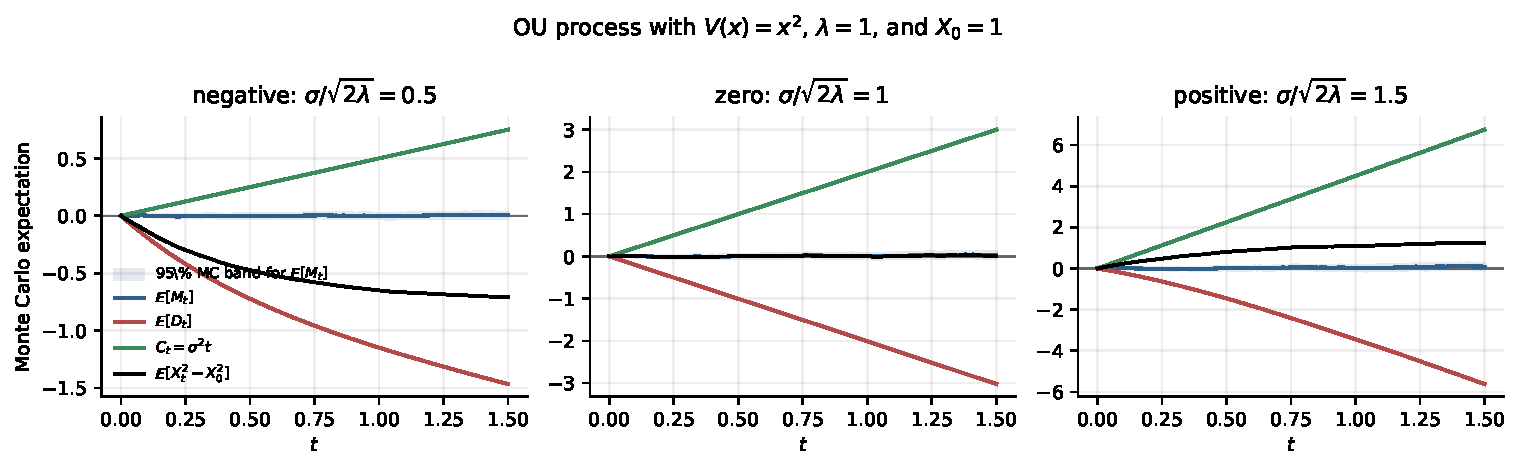
\includegraphics[width=\textwidth]{figures/ou_generator_three_cases.pdf}
  \caption{Monte Carlo expectations from $8000$ Ornstein--Uhlenbeck paths for
  $V(x)=x^2$. The three columns use
  $\sigma/\sqrt{2\lambda}=0.5,1,1.5$. The shaded region is a pointwise
  approximate 95\% Monte Carlo band for $\mathbb E[M_t]$.}
  \label{fig:ou-terms}
\end{figure}

\subsection{Failure of piecewise linearity and success of curvature}

For $f=1$ and $g=\sqrt{2}$ on $[0,1]$, consider a case where want to find a certificate $V$ such that $V(0) = 0$ and $V(1) = 1$.

% the increasing linear candidate
% $V_{\mathrm{PL}}(x)=x$ has
% \[
%   \mathcal{L}V_{\mathrm{PL}}(x)=1>0.
% \]
% More generally, an increasing piecewise-linear certificate must have positive
% slope on some open interval; on that interval its curvature vanishes and
% $\mathcal{L}V=V'>0$. 

A smooth candidate could be:
\[
  V_{\mathcal C^2}(x)=x-\frac{x^2}{2},
\]
the curvature contribution compensates for the positive drift:
\[
  \mathcal{L}V_{\mathcal C^2}(x)
  =(1-x)+\frac12(-1)(2)=-x\leq0.
\]

and indeed $V_{\mathcal C^2}$ is a valid supermartingale certificate.

On the other hand, let's assume $V$ is piecewise linear. 
Then there exists an interval $(x_i, x_{i+1}) \subset [0,1]$ where $V'(x) = a_i > 0$. On that interval, given an $x \in (x_i, x_{i+1})$, the curvature term vanishes, and the generator is
\[
  \mathcal{L}V(x) = V'(x) f(x) + \frac{1}{2} V''(x) g^2(x) = V'(x) f(x) = V'(x) = a_i > 0.
\]

This example motivates the following hypothesis, which we will study in more detail in \autoref{sec:piecewise-quadratic}.

\begin{hypothesis}
  While piecewise linear certificates $V_{\mathrm{PL}}$ are not sufficient to guarantee that $V_{\mathrm{PL}}$ is a supermartingale, \textbf{piecewise quadratic certificates} are sufficient, as the curvature term can compensate for positive drift.
\end{hypothesis}

\begin{figure}[htbp]
  \centering
  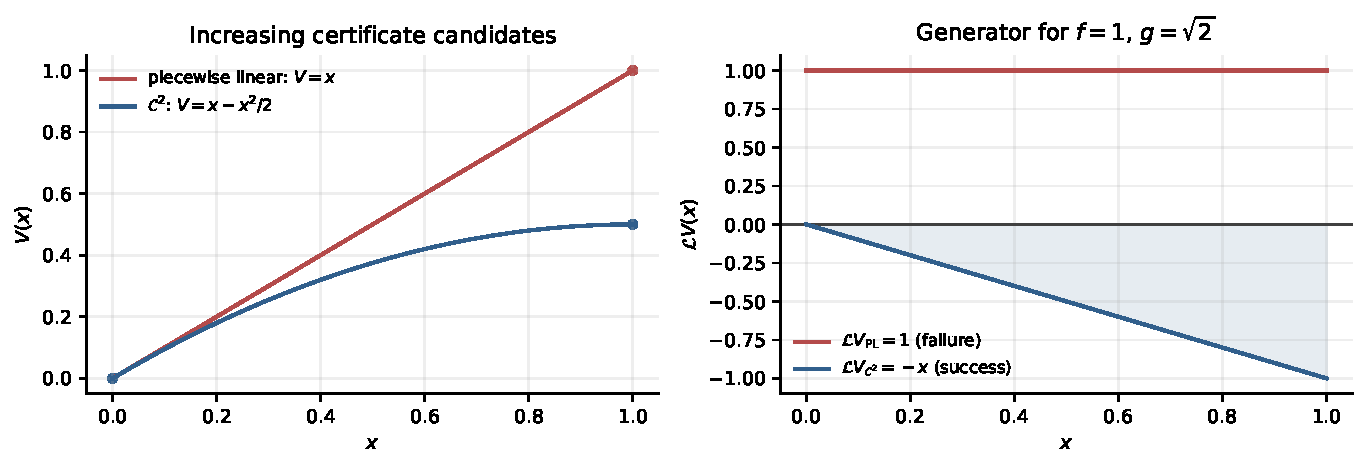
\includegraphics[width=\textwidth]{figures/linear_failure_curvature_success.pdf}
  \caption{An increasing piecewise-linear candidate fails the generator
  condition for $f=1$, $g=\sqrt{2}$, whereas negative curvature makes the
  smooth candidate satisfy it throughout $[0,1]$.}
  \label{fig:linear-vs-curved}
\end{figure}



\subsection{A piecewise $\mathcal{C}^2$ certificate with curvature and a kink}

Finally, let $dX_t=dW_t$ and
\[
  V(x)=
  \begin{cases}
    -\frac12x^2, & x<0,\\
    -x, & x\geq0.
  \end{cases}
\]
Here $D_t=0$, while
\[
  M_t=\int_0^t V'(X_s)\,dW_s,
  \qquad
  C_t=-\frac12\int_0^t\mathbf{1}_{\{X_s<0\}}\,ds,
  \qquad
  K_t=-\frac12L_t^0(X).
\]
Thus $C_t$ decreases while the path lies below zero, and $K_t$ decreases only
when local time accumulates at the kink. Figure~\ref{fig:hybrid-terms} shows
these different mechanisms on the same Brownian realization. The plotted
local time uses an occupation-density approximation with bandwidth $0.06$.

\begin{figure}[htbp]
  \centering
  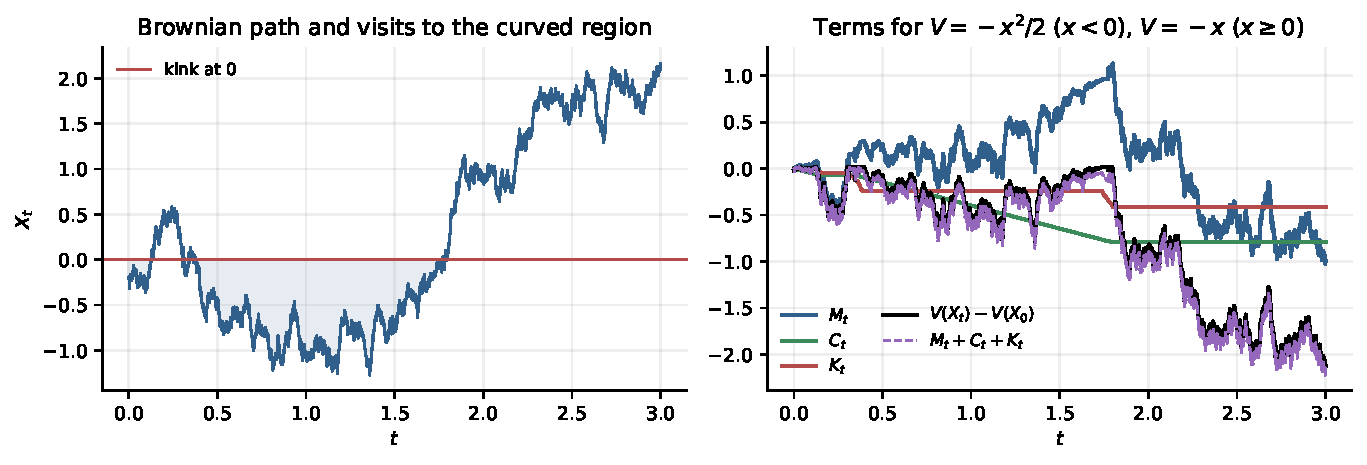
\includegraphics[width=\textwidth]{figures/hybrid_piecewise_c2_terms.pdf}
  \caption{A Brownian realization and the terms for the hybrid piecewise
  $\mathcal C^2$ certificate. The curvature and kink terms are both
  nonincreasing, while the martingale term fluctuates.}
  \label{fig:hybrid-terms}
\end{figure}

\newpage

